\documentclass[11pt,a4paper]{article}
\usepackage[margin=25mm]{geometry}
\usepackage{amsmath,amssymb,graphicx,booktabs,xcolor,xurl,hyperref}
\hypersetup{hidelinks}
\graphicspath{{../artifacts/figures/}}
\title{Harvesting under a Strong Allee Effect: Collapse Thresholds, Hysteresis and Comparison of Constant-Yield vs Proportional-Effort Harvesting, with Physics-Informed Neural Network (PINN) Forward and Inverse Analysis}
\author{Five authors to be filled after task selection}
\date{Mathematical Modelling Group Project, 2026}
\begin{document}
\maketitle
\begin{abstract}
\textbf{SCAFFOLD\_ONLY:} This is an editable structure. Replace with the actual problem, methods, measured results and limitations after all five tasks are complete. No completed scientific result is claimed here.
\end{abstract}
\section{Foundations and Model A: steady populations under a fixed catch}
\label{sec:foundations}

\paragraph{Question.} Suppose the same amount is caught every year. At what population sizes can the stock hold steady, which of these are safe, and how large can the catch be before collapse becomes certain?

\subsection{Scaling}
\label{sec:scaling}
The model has four parameters, but only two combinations of them actually matter. If we measure the population as a fraction of capacity, $x=N/K$, and time in units of $1/r$, $\tau=rt$, the chain rule gives $dN/dt=rK\,dx/d\tau$. Dividing Eq.~\eqref{eq:modelA} by $rK$ then leaves
\begin{equation}
\frac{dx}{d\tau}=f(x)=G(x)-q,\qquad G(x)=x(1-x)\Bigl(\frac{x}{a}-1\Bigr),
\label{eq:A_dimless}
\end{equation}
where $a=A/K$ is the Allee threshold as a fraction of capacity and $q=H/(rK)$ is the scaled catch. In the same way the logistic model becomes $dx/d\tau=x(1-x)-q$, and Model B becomes $dx/d\tau=G(x)-ex$ with $e=h/r$. Any result can be turned back into real units using $N=Kx$, $t=\tau/r$ and $H=rKq$. All examples in this section use $a=0.2$.

\subsection{Steady states and stability}
A steady state, or equilibrium, is a population $x_e$ at which growth and catch cancel out, so that $f(x_e)=0$ and nothing changes. To decide whether it is stable, we look at the sign of $f$ just on either side of it \cite{strogatz2015nonlinear}. If $f$ is positive just below $x_e$ and negative just above, a population nudged slightly away is pulled back, and the state is \emph{stable}. If the signs are the other way round, small nudges grow and the state is \emph{unstable}. If $f$ has the same sign on both sides, the state attracts from one side and repels on the other, and we call it \emph{semistable}. Wherever $f'(x_e)\neq0$ this agrees with the familiar derivative test ($f'<0$ stable, $f'>0$ unstable), but at a point where $f'(x_e)=0$ only the signs can settle the question.

\paragraph{Logistic baseline.} It helps to start with the model without an Allee effect, $f(x)=x(1-x)-q$. For $q<\tfrac14$ it has two steady states,
\begin{equation}
x_\pm=\tfrac12\bigl(1\pm\sqrt{1-4q}\bigr).
\end{equation}
The upper one is stable. The lower one is unstable, a threshold that exists only because of the catch. As $q$ grows the two move towards each other and meet at $x=\tfrac12$ when $q=\tfrac14$, which gives the well-known maximum constant catch $H_c=rK/4$ \cite{brauer2012mathematical}. Any larger catch drives every population to zero. With no catch at all, zero is unstable, so even a very small population grows back.

\subsection{Model A: the growth curve and the maximum catch}
With the Allee factor included, the growth curve $G$ is negative between $0$ and $a$ and positive between $a$ and $1$. In other words, it dips below zero when the population is small and then rises into a single hill. The top of the hill is where $G'(x)=0$, which works out to $3x^2-2(1+a)x+a=0$. Taking the larger root,
\begin{equation}
x^*=\frac{1+a+\sqrt{1-a+a^2}}{3},\qquad q_c=G(x^*).
\label{eq:fold}
\end{equation}
Steady states are the points where the horizontal line at height $q$ meets this curve, which leaves four cases.
\begin{itemize}
\item With no catch ($q=0$) there are three steady states. Both $x=0$ and $x=1$ are stable, while $x=a$ in between is unstable: this is the minimum viable population. Unlike the logistic model, extinction is now a stable outcome.
\item For a moderate catch ($0<q<q_c$) the line cuts the hill twice, at an unstable $x_-$ between $a$ and $x^*$ and a stable $x_+$ between $x^*$ and $1$. A population starting below $x_-$ dies out, while one starting above it settles at $x_+$.
\item At $q=q_c$ the line just touches the top of the hill, and the two states merge into a single semistable point at $x^*$, called the \emph{fold}.
\item For $q>q_c$ the line never meets the hill, and every population collapses.
\end{itemize}

Once there is any catch at all, zero stops being a steady state, because $f(0)=-q<0$. A declining population therefore reaches zero in finite time, and we stop the simulation at that point. For $a=0.2$ we get $x^*\approx0.706$ and $q_c\approx0.525$. With $r=0.5$ per year and $K=1000$ t, the largest catch the stock can sustain is about $263$ t/yr, at a stock of about $706$ t.

\subsection{Finding the steady states numerically}
To compute the steady states for a given catch, we use the shape of $G$ directly:
\begin{enumerate}
\item Compute $x^*$ and $q_c$ from Eq.~\eqref{eq:fold}.
\item If $q>q_c$ there is no positive steady state, and if $q=q_c$ the only one is $x^*$.
\item If $0<q<q_c$, $f$ changes sign exactly once between $a$ and $x^*$ and once between $x^*$ and $1$. Each root is found with Brent's method, a standard root finder that repeatedly shrinks an interval containing a sign change.
\item Each root is then labelled stable or unstable from the sign of $f$ on either side.
\end{enumerate}
For $a=0.2$ and $q=0.3$ this gives $x_-=0.4431$ (unstable) and $x_+=0.9063$ (stable). Very close to $q_c$ the two roots become nearly equal, and if floating-point arithmetic cannot tell them apart, the code reports an error instead of quietly merging them.

\subsection{Growth curves and the branch diagram}
Figure~\ref{fig:wp01_geometry} puts this picture on paper. In the logistic panels a threshold only appears once fishing starts. Model A already has one at $x=a$ with no catch, and fishing pushes it higher. Once the catch exceeds $q_c$, the line passes above the whole hill.

\begin{figure}[!htbp]
\centering
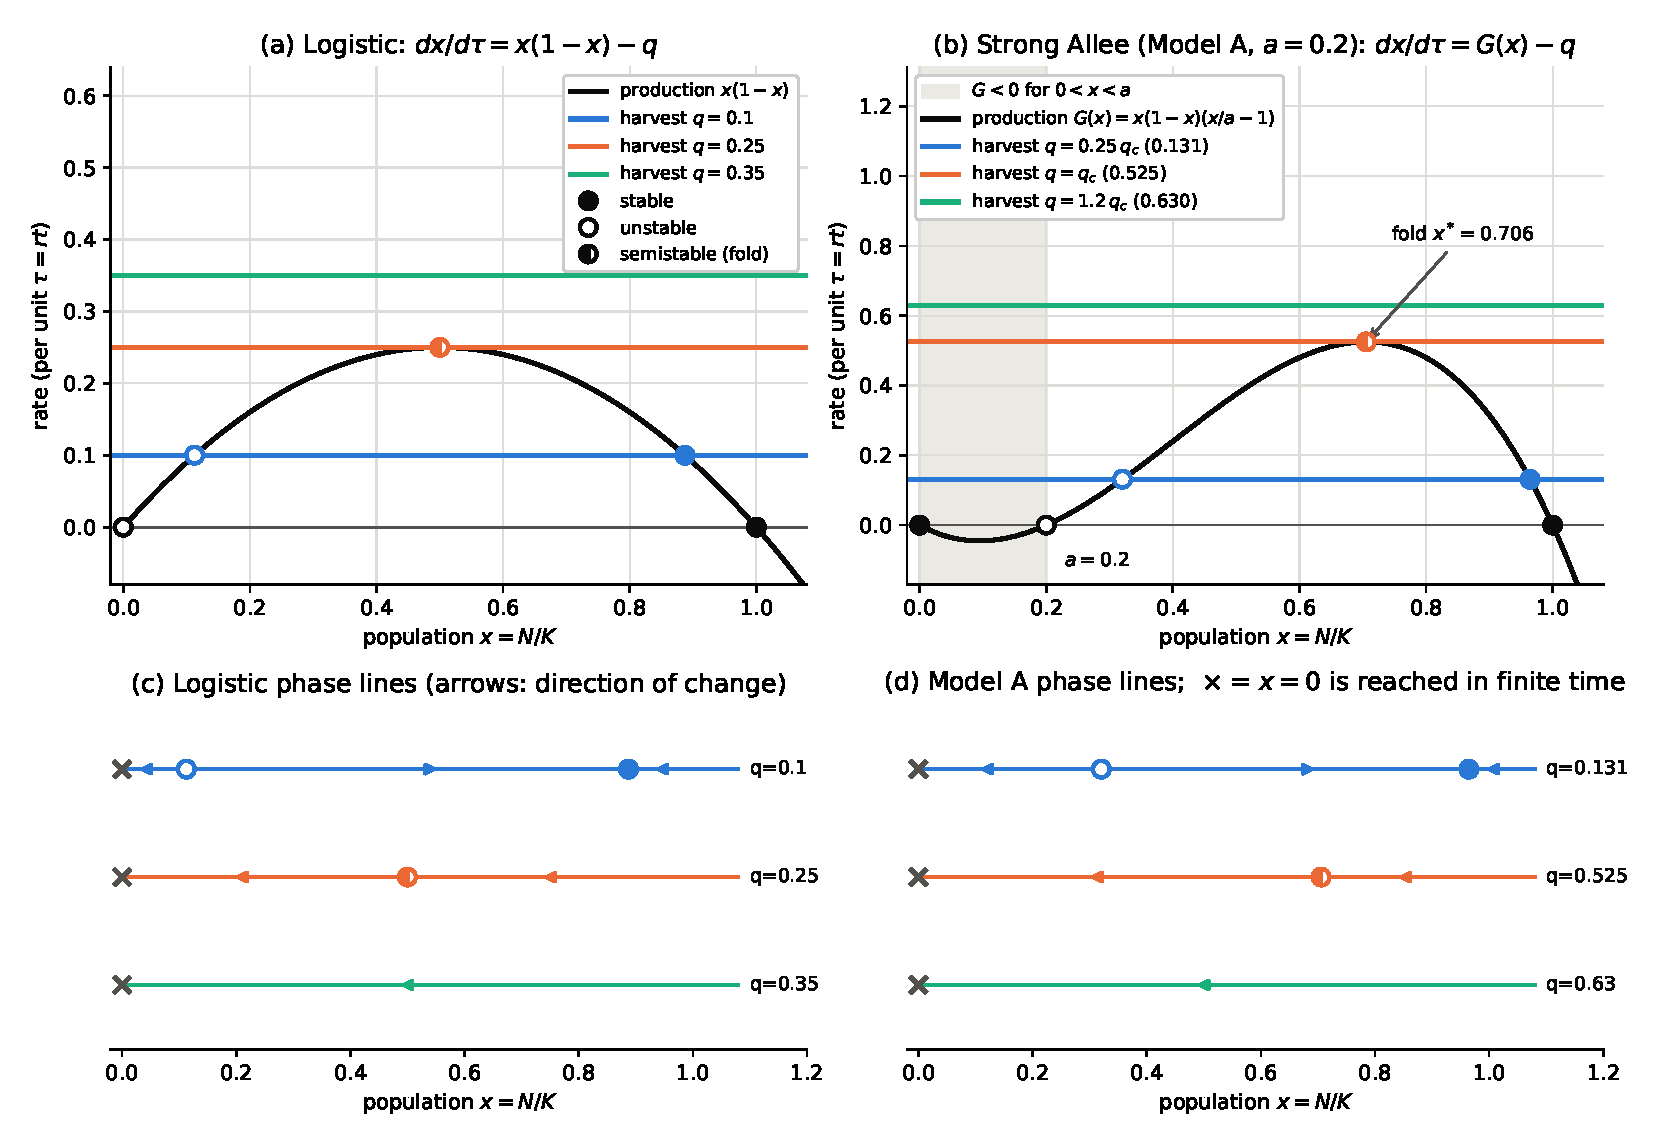
\includegraphics[width=0.85\textwidth]{wp01_logistic_vs_allee}
\caption{Growth curves and phase lines. (a)~Logistic growth $x(1-x)$ with catch lines. (b)~Strong-Allee growth $G(x)$ for $a=0.2$, with catches of $0.25q_c$, $q_c$ and $1.2q_c$. Filled, open and half-filled circles mark stable, unstable and semistable states. (c,d)~Phase lines: arrows show whether the population grows or shrinks, and $\times$ marks $x=0$, which is reached in finite time when $q>0$.}
\label{fig:wp01_geometry}
\end{figure}

Plotting the steady states against the catch gives the branch diagram in Figure~\ref{fig:wp01_branches}. As the catch increases, the stable branch and the collapse threshold approach each other and meet at the fold $(q_c,x^*)$. The distance $x_+-x_-$ between them is the stock's safety margin, and near the fold it shrinks like $\sqrt{q_c-q}$.

\begin{figure}[!htbp]
\centering
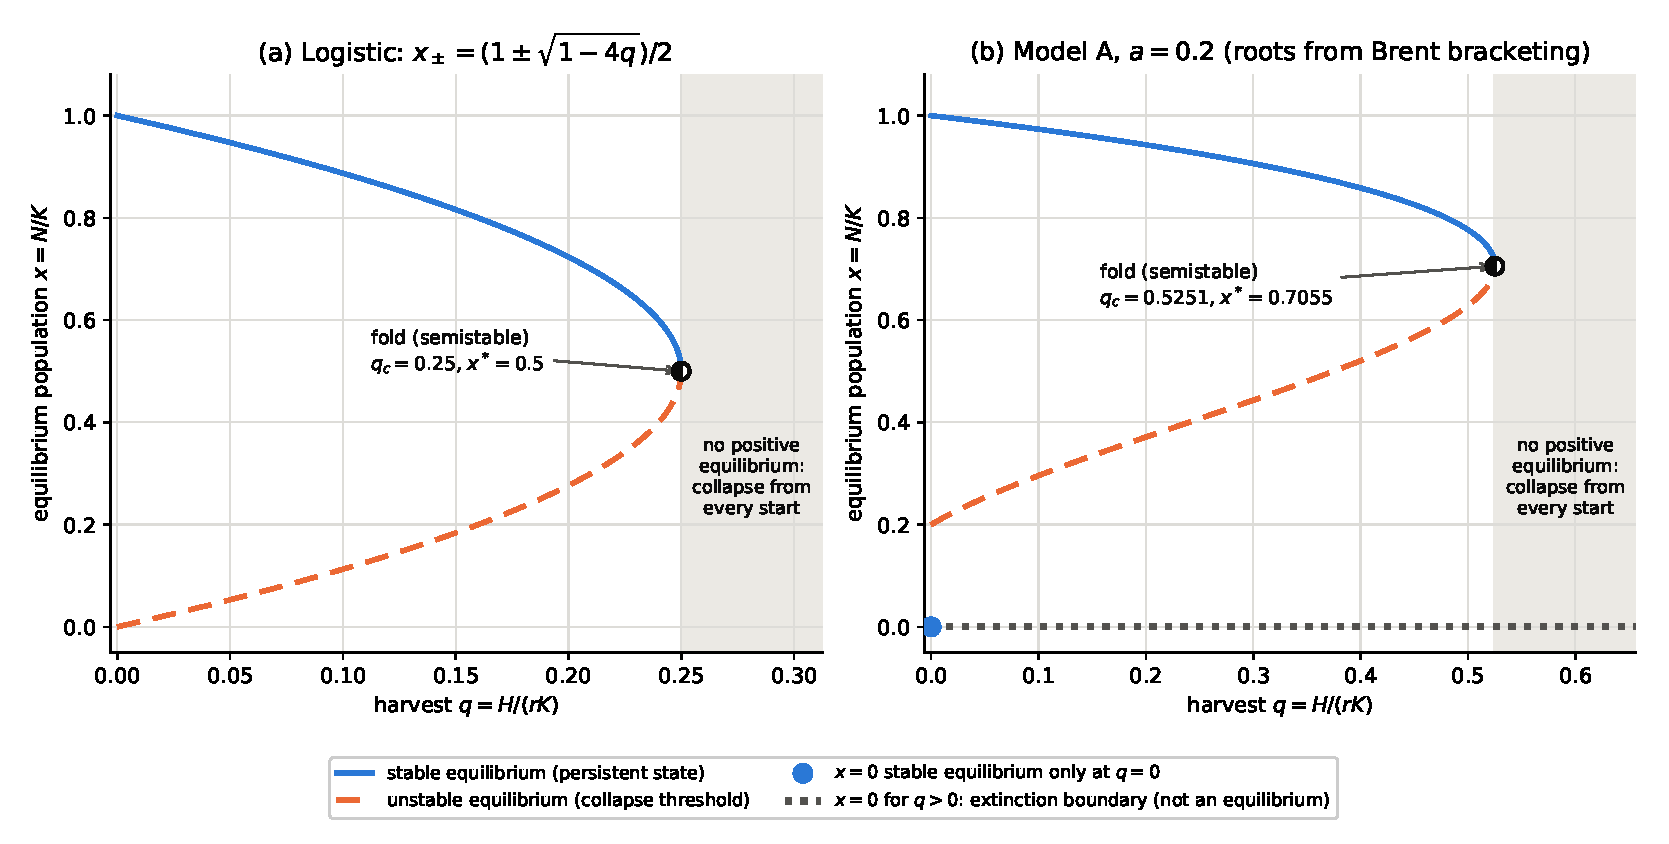
\includegraphics[width=0.92\textwidth]{wp01_model_a_branches}
\caption{Steady states against the scaled catch $q=H/(rK)$. (a)~Logistic. (b)~Model A with $a=0.2$. Solid lines are stable, dashed lines unstable, and the half-filled circle is the semistable fold. The shaded region $q>q_c$ has no positive steady state. In (b) the dotted line at $x=0$ marks extinction, which is not a steady state when $q>0$.}
\label{fig:wp01_branches}
\end{figure}

\subsection{Checking stability by simulation}
As a check on these labels, we took $q=0.3$, started the population $\delta=0.01$ above and below each steady state, and solved the equation with a standard Runge--Kutta solver (RK45 \cite{scipy_solve_ivp}) that stops at $x=0$. Both starts near $x_+$ return to it. The start just above $x_-$ climbs back up to $x_+$, while the one just below falls and reaches zero at $\tau\approx2.9$ (Figure~\ref{fig:wp01_perturb}). This is exactly what the sign analysis predicted.

\begin{figure}[!htbp]
\centering
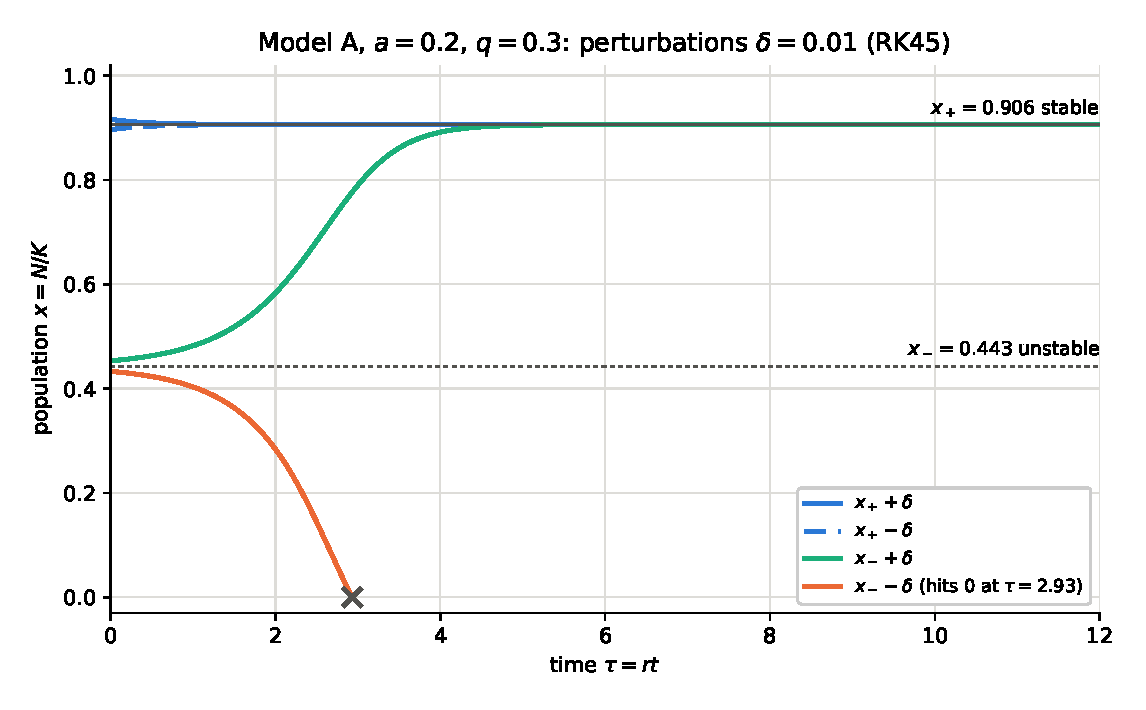
\includegraphics[width=0.62\textwidth]{wp01_model_a_perturbations}
\caption{Simulation check for Model A with $a=0.2$ and $q=0.3$, starting $\delta=0.01$ above and below each steady state.}
\label{fig:wp01_perturb}
\end{figure}

\FloatBarrier
\subsection{Result and limitations}
\paragraph{Main result.} As the fixed catch rises, the safe steady state and the collapse threshold draw closer and finally merge at the maximum catch $q_c$. A disturbance only causes collapse if it pushes the population below the threshold, that is, if it is larger than the gap between the two. Since this gap closes at $q_c$, fishing near the maximum leaves almost no room for a bad year.

\paragraph{Limitations.} The model ignores randomness, which matters most near the threshold. The cubic growth law is a simple phenomenological choice, the parameters are held constant, and the full catch is assumed to be taken whenever $N>0$. All numbers are illustrative rather than measured from a real stock.
\section{Model B, comparison and harvesting history}
\textbf{SCAFFOLD\_ONLY:} B roots/stability; fair A/B comparisons; up/down ramp with state carry-over; explicit restocking; no invented automatic recovery.

Replace this template with derivations, algorithms, labelled figures/tables, interpretation, limitations and verified references from WP02.


\section{Critical Harvesting Rates and Extinction Analysis}
\label{sec:wp03}

In Sections~\ref{sec:foundations} and~\ref{sec:wp02}, we studied the
equilibrium points and stability of Models A and B. We now calculate
the critical harvesting rates, examine how the initial population
affects survival, and determine the time to extinction when a
population collapses. We also investigate slow decline near the
critical harvesting rate.

We use the dimensionless variables introduced earlier:
\[
x=\frac{N}{K},\qquad
\tau=rt,\qquad
a=\frac{A}{K},\qquad
q=\frac{H}{rK},\qquad
e=\frac{h}{r}.
\]
The two harvesting models are
\begin{align}
\text{Model A:}\qquad x' &= G(x)-q,\\
\text{Model B:}\qquad x' &= G(x)-ex,
\end{align}
where
\[
G(x)=x(1-x)\left(\frac{x}{a}-1\right),
\qquad x'=\frac{dx}{d\tau}.
\]

\subsection{Critical Harvesting Rates}
\label{sec:wp03-thresholds}

\paragraph{Model A: Constant harvesting.}
At a positive equilibrium, natural growth balances the fixed
catch: $G(x)=q$. The largest constant catch that can be balanced
is therefore the maximum of $G(x)$ for $x\geq0$.
Expanding and differentiating gives
\[
G(x)=-\frac{x^3}{a}+\frac{(1+a)x^2}{a}-x,
\qquad
G'(x)=\frac{-3x^2+2(1+a)x-a}{a}.
\]
Setting $G'(x)=0$ gives
\[
x=\frac{1+a\pm\sqrt{1-a+a^2}}{3}.
\]
The larger stationary point lies between $a$ and $1$.
Writing it as $x_*$, we have
\[
x_*=\frac{1+a+\sqrt{1-a+a^2}}{3},
\qquad
G''(x_*)=-\frac{2\sqrt{1-a+a^2}}{a}<0.
\]
Thus the critical constant catch is
\begin{equation}
q_c=G(x_*),\qquad H_c=rKq_c.
\label{eq:wp03-critical-a}
\end{equation}
The corresponding population in the original units is
\[
N_*=Kx_*=
\frac{K+A+\sqrt{K^2-KA+A^2}}{3}.
\]

\paragraph{Model B: Proportional harvesting.}
At a positive equilibrium, $G(x)=ex$. Dividing by $x>0$ gives
\[
e=\frac{G(x)}{x}
=(1-x)\left(\frac{x}{a}-1\right)=P(x).
\]
Here we maximise growth per unit population, rather than
total growth. Since
\[
P'(x)=\frac{1+a-2x}{a},
\qquad P''(x)=-\frac{2}{a}<0,
\]
the maximum occurs at $x=(1+a)/2$. Hence
\begin{equation}
e_c=\frac{(1-a)^2}{4a},
\qquad
h_c=\frac{r(K-A)^2}{4AK}.
\label{eq:wp03-critical-b}
\end{equation}

Above their respective critical harvesting rates, neither model
has a positive equilibrium. Below these rates, positive
equilibria exist, but the initial population still determines
whether the population survives.

For the numerical examples in this section, we use
$r=0.7$, $K=100$ and $A=20$. We obtain
\[
N_*\approx70.55050,\qquad
H_c\approx36.75966,\qquad h_c=0.56.
\]
For comparison, the standard logistic model with constant
harvesting has $H_{c,\mathrm{logistic}}=rK/4=17.5$.
However, the logistic and Allee models have different growth
functions. The larger critical harvesting rate does not mean
that populations with a strong Allee effect are always more
resistant to collapse. Also, $H$ and $h$ have different
units, so their numerical values cannot be compared directly.

We checked the analytical thresholds by independently
maximising the corresponding growth functions numerically.

\subsection{Initial Population and Basins of Attraction}
\label{sec:wp03-basins}

Even below the critical harvesting rate, a population may
collapse if its initial size is too small. A \emph{basin of
attraction} is the set of initial populations that approach
the same long-term state.

For Model A with $0<q<q_c$, there are two positive
equilibria, $x_-<x_+$. The sign of $G(x)-q$ is negative
below $x_-$, positive between the roots, and negative
above $x_+$. Therefore $x_-$ is unstable and $x_+$
is stable. A population starting below $x_-$ reaches
zero, whereas a population starting above it approaches
$x_+$.

For Model B, the positive equilibria are
\[
x_\pm=
\frac{1+a\pm\sqrt{(1-a)^2-4ae}}{2},
\qquad 0\leq e<e_c.
\]
The lower equilibrium is unstable and the upper one is
stable. Model B also has a stable zero equilibrium:
if $f_B(x)=G(x)-ex$, then
\[
f'_B(0)=-(1+e)<0.
\]

At the critical harvesting rate, the two positive
equilibria merge at a \emph{fold}. For Model A this
occurs at $x_*$, and for Model B at $(1+a)/2$.
The merged equilibrium attracts populations from
above but not from below. This one-sided behaviour
is called \emph{semistability}.

Table~\ref{tab:basins} summarises the outcomes.

\begin{table}[htbp]
\centering
\small
\caption{Long-term outcomes for positive initial populations.
For below-critical harvesting, the harvest is positive.
A population starting exactly at an equilibrium remains there.}
\label{tab:basins}
\begin{tabular}{p{0.17\linewidth}p{0.36\linewidth}p{0.36\linewidth}}
\toprule
\textbf{Harvesting} & \textbf{Model A} & \textbf{Model B}\\
\midrule
Zero
& For $x_0<a$, approaches zero; for $x_0>a$, approaches $1$.
& Same behaviour as Model A.\\
Below critical
& For $x_0<x_-$, reaches zero; for $x_0>x_-$, approaches $x_+$.
& For $x_0<x_-$, approaches zero; for $x_0>x_-$, approaches $x_+$.\\
At critical
& Below the merged root, reaches zero; above it, approaches the merged root.
& Below the merged root, approaches zero; above it, approaches the merged root.\\
Above critical
& Every finite $x_0>0$ reaches zero.
& Every $x_0>0$ approaches zero.\\
\bottomrule
\end{tabular}
\end{table}

With zero harvesting, $x_0=a$ is also an equilibrium.
For Model A with $q>0$, however,
$G(0)-q=-q<0$: zero is a boundary at which we
stop the physical solution, not an equilibrium of
the original ODE. A population on a collapsing
trajectory reaches this boundary in finite time.
Under Model B, a declining positive population
approaches zero asymptotically instead.

Figure~\ref{fig:wp03_basins} shows the basin diagrams.
The blue regions show initial conditions leading to
a positive equilibrium. The orange region in Model A
shows finite-time extinction, while the yellow region
in Model B shows asymptotic decline. The lower
equilibrium separates collapse from persistence below
the critical harvesting rate. We classify the basins
from the signs of the equations rather than simply
using the value at the end of a finite simulation.
Conditions extremely close to an unstable or merged
equilibrium are marked unresolved when rounding
prevents a reliable classification.

\begin{figure}[htbp]
\centering
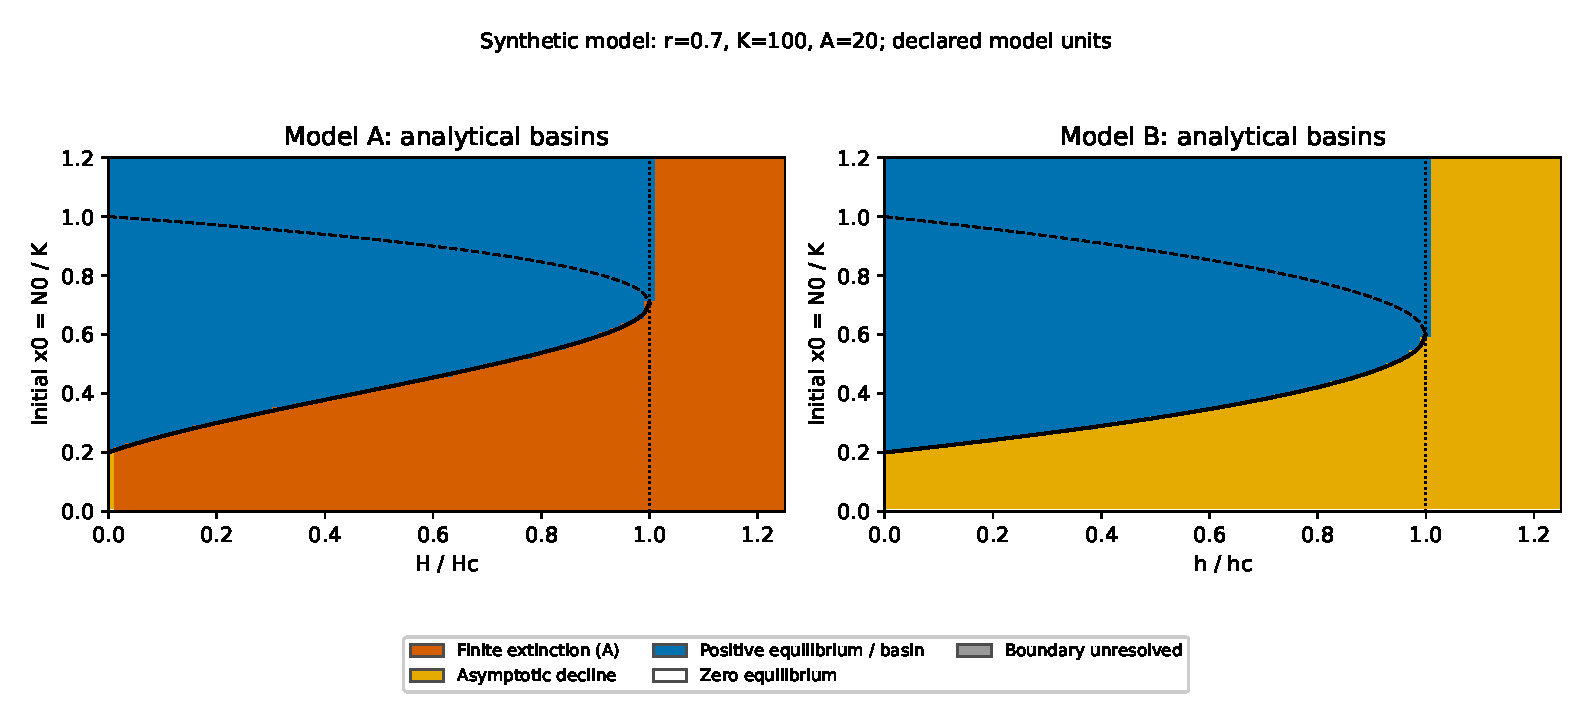
\includegraphics[width=\linewidth]{wp03_basins}
\caption{Basins of attraction for Models A and B with $a=0.2$.
The horizontal axis in each panel is the harvest divided by
that model's critical rate; the vertical axis is the initial
population $x_0=N_0/K$. Solid curves mark lower equilibria,
dashed curves mark upper equilibria, and vertical dotted
lines mark the critical harvesting rates.}
\label{fig:wp03_basins}
\end{figure}

\subsection{Time to Extinction}
\label{sec:wp03-extinction}

For a Model A trajectory that reaches zero, the
extinction time follows from separation of variables:
\[
\frac{dx}{d\tau}=G(x)-q,
\qquad
\tau_{\mathrm{ext}}
=\int_{x_0}^{0}\frac{dx}{G(x)-q}
=\int_0^{x_0}\frac{du}{q-G(u)}.
\]
To express this in the original units, recall that
\[
x=\frac{N}{K},\qquad
\tau=rt,\qquad
q-G(x)=\frac{H-g(N)}{rK},
\]
where
\[
g(N)=rN\left(1-\frac{N}{K}\right)
\left(\frac{N}{A}-1\right).
\]
Since $dx=dN/K$, the substitution gives
\[
\tau_{\mathrm{ext}}
=r\int_0^{N_0}\frac{dN}{H-g(N)}.
\]
Thus the dimensional extinction time is
\begin{equation}
t_{\mathrm{ext}}
=\frac{\tau_{\mathrm{ext}}}{r}
=\int_0^{N_0}\frac{dN}{H-g(N)}.
\label{eq:wp03-extinction}
\end{equation}

This integral gives a finite extinction time only
when the trajectory reaches zero without encountering
an equilibrium. We therefore classify the initial
condition before evaluating it. If an equilibrium
lies along the path to zero, the denominator
vanishes and the integral cannot be used to assign
a finite extinction time.

For $q>q_c$, we have $G(x)\le q_c$ for all $x\ge0$.
Consequently,
\[
q-G(x)\ge q-q_c>0,
\qquad
\tau_{\mathrm{ext}}\le\frac{x_0}{q-q_c}.
\]
Every finite positive initial population therefore
reaches zero in finite time for Model A above its
critical constant catch. At $q=q_c$, a start below
$x_*$ still reaches zero; a start above $x_*$
approaches the merged equilibrium instead.

For Model B, a positive trajectory cannot reach
its zero equilibrium in finite time because the
ODE is smooth and solutions are unique. The same
holds for Model A when $q=0$. A numerical time
to a small positive cutoff is not an exact
extinction time in either of these situations.

We evaluate the extinction-time integral using
numerical quadrature \cite{scipy_quad}. Close to
a basin boundary or the fold, its denominator
can become small and the calculation requires
care. Our implementation uses changes of variable
near difficult points. These numerical estimates
are checked independently below.

\subsection{Numerical Method and Accuracy Checks}
\label{sec:wp03-validation}

We solve the population ODEs using SciPy's RK45
method, based on the adaptive Dormand--Prince
Runge--Kutta pair of orders five and four
\cite{dormand1980family,scipy_solve_ivp}.
The difference between the two estimates is used
to adjust the step size. Our reference settings
are relative tolerance $10^{-9}$, absolute
tolerance $10^{-11}$ and maximum dimensionless
step size $0.1$.

For Model A under positive catch, the solver
stops at the first downward crossing of zero.
We do not continue the original ODE into
negative populations.

For six Model A extinction cases, we compare
the separated integral with RK45 at two tolerances
and with the independent DOP853 method. The cases
cover harvesting below, at and above the critical
rate, with initial populations chosen on
extinction trajectories. We use the acceptance
condition
\[
|\Delta\tau|
\le 2\times10^{-7}
+5\times10^{-7}\tau_{\mathrm{ext}}.
\]
Table~\ref{tab:event_checks} lists each case.
Here $x_0=N_0/K$, and $q/q_c$ is the fraction
of the critical constant catch.

\begin{table}[htbp]
\centering
\footnotesize
\setlength{\tabcolsep}{4pt}
\caption{Six Model A extinction-time checks.
The largest difference is the maximum absolute
difference between the quadrature result and
the tested ODE integrations, in dimensionless time.}
\label{tab:event_checks}
\begin{tabular}{ccccc}
\toprule
$q/q_c$ & $x_0$ & $\tau_{\mathrm{ext}}$
& $\max|\Delta\tau|$ & Tolerance\\
\midrule
0.25 & 0.10000 & 0.6198 & $2.3\times10^{-10}$ & $5.1\times10^{-7}$\\
0.75 & 0.35769 & 0.9957 & $1.6\times10^{-9}$ & $7.0\times10^{-7}$\\
1.00 & 0.56440 & 1.9303 & $6.4\times10^{-9}$ & $1.2\times10^{-6}$\\
1.01 & 1.10000 & 19.9106 & $4.6\times10^{-8}$ & $1.0\times10^{-5}$\\
1.05 & 1.10000 & 8.6537 & $3.8\times10^{-8}$ & $4.5\times10^{-6}$\\
1.20 & 1.10000 & 4.0293 & $3.9\times10^{-8}$ & $2.2\times10^{-6}$\\
\bottomrule
\end{tabular}
\end{table}

All six cases passed, with the largest recorded
difference approximately $4.56\times10^{-8}$
in dimensionless time. This supports numerical
agreement for the tested cases, rather than a
global accuracy guarantee.

Figure~\ref{fig:wp03_extinction} shows Model A
extinction times for different initial populations
and constant catches. In the left panel, the time
grows as the starting population approaches the
unstable equilibrium from below. Above that
boundary, the population persists and there is
no finite extinction time to plot.

The right panel fixes the initial population and
varies the constant catch. For a population that
reaches zero, a larger catch produces a shorter
extinction time. When the initial population lies
above the fold population, extinction occurs only
for $H>H_c$, and the time can be very large just
above this threshold. Both vertical axes are
logarithmic. The underlying analysis contains
427 records, including cases without a reported
finite extinction time.

\begin{figure}[htbp]
\centering
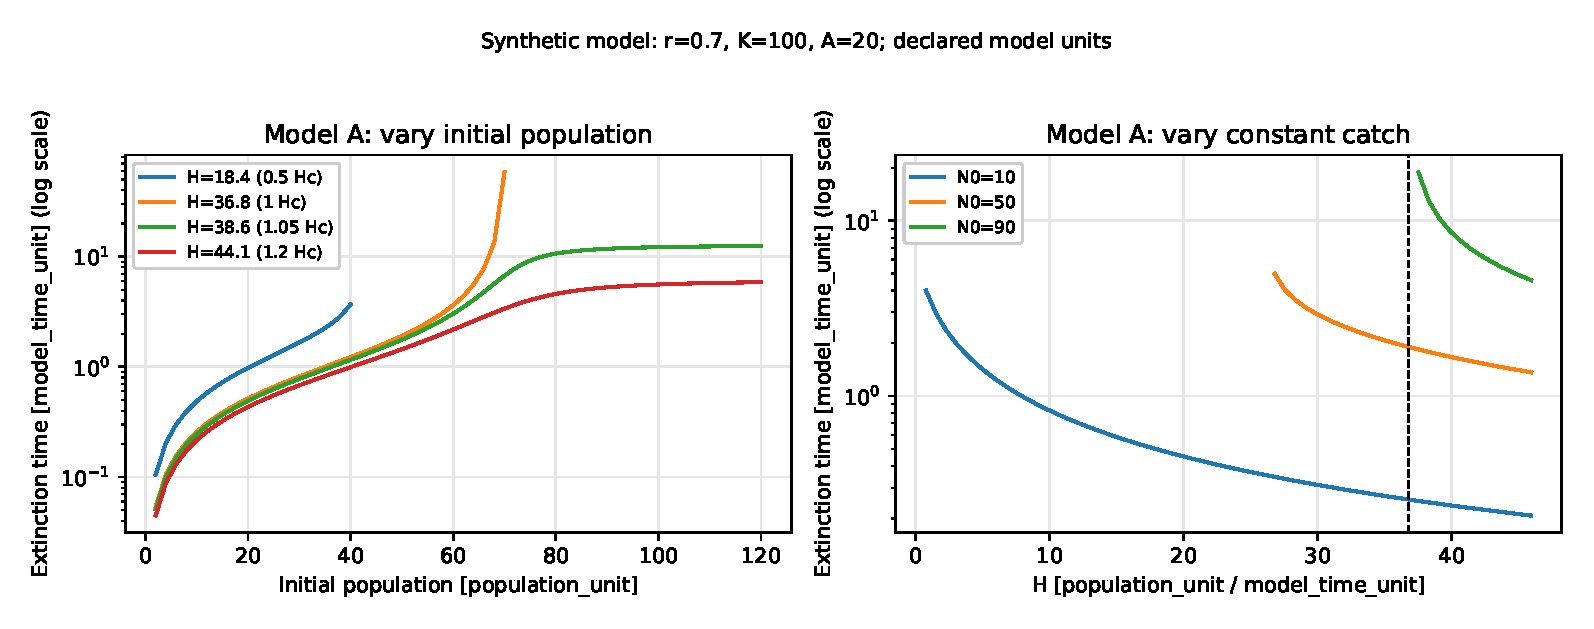
\includegraphics[width=\linewidth]{wp03_extinction}
\caption{Model A extinction time against initial population
(left) and constant harvesting rate (right), with
$r=0.7$, $K=100$ and $A=20$. Both vertical axes
are logarithmic. Gaps indicate cases without a
reported finite extinction time; the dashed line
on the right marks $H_c$.}
\label{fig:wp03_extinction}
\end{figure}

\subsection{Slow Decline Near the Critical Harvesting Rate}
\label{sec:wp03-bottleneck}

Extinction need not happen quickly when $q$ is only
slightly larger than $q_c$. Although no positive
equilibrium remains, natural growth almost balances
the constant catch near the former equilibrium
population $x_*$. The net decline is small there,
so the population can spend a long time in this
region before falling to zero. This slow passage
is called a \emph{bottleneck}.

Figure~\ref{fig:wp03_bottleneck} shows three
trajectories starting at $x_0=1.1$, with
$a=0.2$ and harvesting rates just above $q_c$.
The closer the catch is to its critical value,
the longer the delay. Each trajectory ends at
its calculated zero event. We report this
numerical behaviour without fitting a separate
asymptotic scaling law.

\begin{figure}[htbp]
\centering
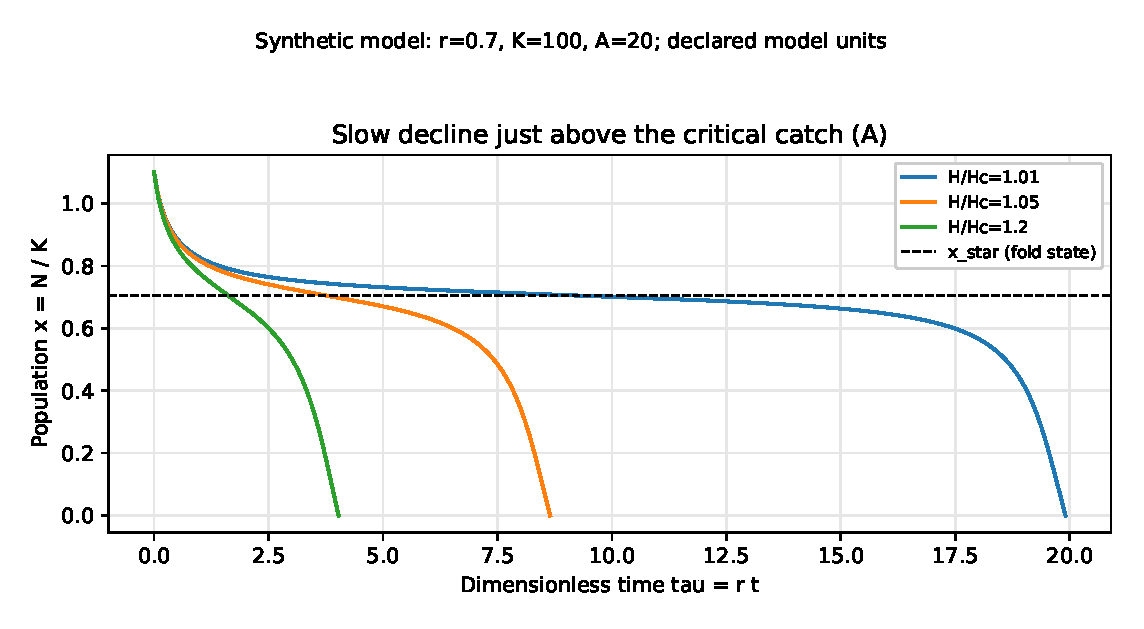
\includegraphics[width=0.9\linewidth]{wp03_bottleneck_core}
\caption{Model A trajectories slightly above the
critical constant catch, with $a=0.2$ and $x_0=1.1$.
Time and population are dimensionless. The dashed
line shows the population at the former fold.
Each curve ends when the population reaches zero.}
\label{fig:wp03_bottleneck}
\end{figure}

\subsection{Synthetic Reference Data and Limitations}
\label{sec:reference}

We also generated six clean synthetic reference
trajectories using RK45. Each contains 101 sampled
population values, giving 606 values in total.
For each model, the three cases are regular
persistence, behaviour near the critical harvesting
rate, and decline or extinction. The Model A
declining case reaches zero in finite time,
whereas the Model B declining case approaches
zero asymptotically.

The generating parameters, initial populations
and solver settings are recorded in the project
configuration files. The six cases are named
\texttt{a\_regular}, \texttt{a\_near\_fold},
\texttt{a\_extinction}, \texttt{b\_regular},
\texttt{b\_near\_fold} and \texttt{b\_decline}.
All six passed comparisons with DOP853 and
tighter-tolerance RK45 integrations.

Figure~\ref{fig:wp03_reference} shows these
reference trajectories. The complete data-generation
scripts, configurations and numerical results
are available in our
\href{https://github.com/devam2006/mm-allee-harvesting}
{GitHub project repository}.

\begin{figure}[htbp]
\centering
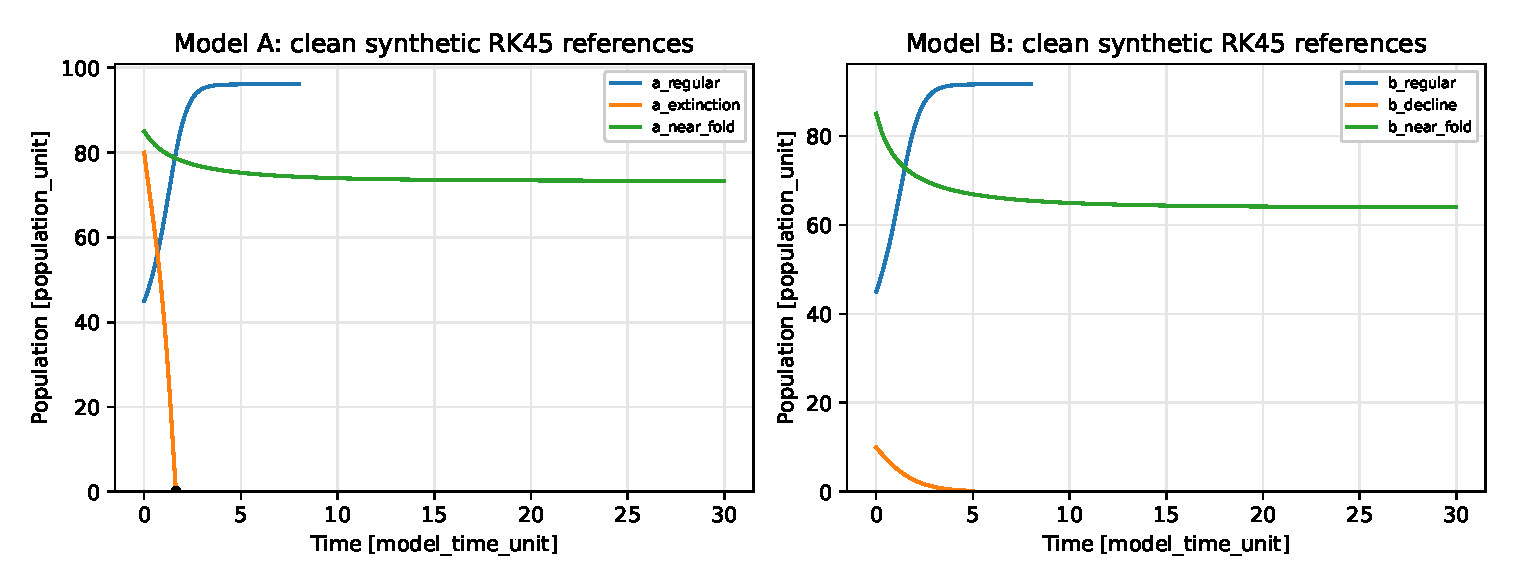
\includegraphics[width=\linewidth]{wp03_rk45_reference}
\caption{Six synthetic RK45 reference trajectories
for Models A and B, showing regular persistence,
near-critical behaviour and decline or extinction.}
\label{fig:wp03_reference}
\end{figure}

These trajectories form an early numerical
reference dataset. The forward PINN experiments
use separately generated numerical reference
solutions for evaluation, while the inverse
experiments use their own observation, noise
and data-splitting procedures. Any zero values
stored after a Model A extinction event represent
an absorbing extinction convention, not a
continuation of the original ODE with constant catch.

\paragraph{Main result.}
Both the harvesting rate and initial population
matter for survival. Positive constant harvesting
can produce finite-time extinction, whereas
declining positive populations under proportional
harvesting approach zero asymptotically.
Collapse can also be delayed near the critical
constant harvesting rate.

\paragraph{Limitations.}
The calculations assume constant parameters
and a well-mixed population, without environmental
randomness, age structure or time delays. All
trajectories are synthetic. The critical rates
and extinction times are consequences of the
specified models, not predictions for a
particular real-world population.

\section{Forward PINNs}
\textbf{SCAFFOLD\_ONLY:} Differentiable network and residual; initial condition/physics loss; optimiser/collocation algorithm; both models and independent solver errors/runtime.

Replace this template with derivations, algorithms, labelled figures/tables, interpretation, limitations and verified references from WP04.

\section{Inverse PINNs and validation}
\textbf{SCAFFOLD\_ONLY:} Identifiable staged unknowns; noisy observations; ODE least-squares baseline; held-out prediction; near-collapse failures; AI/data acknowledgement.

Replace this template with derivations, algorithms, labelled figures/tables, interpretation, limitations and verified references from WP05.

\section{Conclusions and limitations}
\textbf{SCAFFOLD\_ONLY:} Summarise only supported analytical and numerical findings. State the synthetic-data limitation, inverse identifiability limitation and all relevant PINN failures.
\section{Contributions and acknowledgements}
\textbf{SCAFFOLD\_ONLY:} List five actual authors and their chosen task contributions. Consolidate actual AI platforms/roles from docs/AI\_USAGE.md and sources/data/figure acknowledgements. Every author must verify the final text.
\bibliographystyle{plain}
\bibliography{references}
\end{document}
